\section{Research Methodology}

\subsection{Data Collection and Setup}
The data acquisition phase was conducted using a Google Pixel 9a smartphone camera. To ensure
a comprehensive morphological analysis, images of the mangoes were captured from six
distinct viewing angles: Side A, Side B, Top, Bottom, Front, and Back. These varying
orientations dictate the visible surface area and features of the fruit, necessitating the
creation of orientation-specific pipelines for the subsequent ripeness and morphology
models.

Ground truth measurements were meticulously recorded for each sample to supervise the
machine learning models. The procedure included the following steps:
\begin{enumerate}
    \item \textbf{Dimension Measurement:} The absolute height, width, and thickness of the
mango, as well as its extracted bone (stone), were measured using standard rulers.
    \item \textbf{Weight Measurement:} The mass of the whole mango and its extracted bone
    were recorded using a highly sensitive digital weighing scale (see
    Fig.~\ref{fig:weigh_setup}). For ripe samples, the extracted bones were air-dried prior
to weighing to eliminate excess moisture and ensure an accurate reading.
    \item \textbf{Volume Measurement:} The volume of both the mango and the bone was empirically determined using the Archimedes water displacement method in a graduated beaker (see Fig.~\ref{fig:water_disp}).
    \item \textbf{Phase Labeling:} The mangoes were binary-classified into two physiological phases: `ripe' and `unripe'. This classification was determined by inspecting the internal flesh content; mangoes with fully yellow, moist flesh were labeled as ripe, while others were labeled as unripe. This distinction is critical because ripeness influences the density and weight-to-volume relationships \cite{fruitDensity}.
\end{enumerate}

\begin{figure}[htbp]
    \centering
    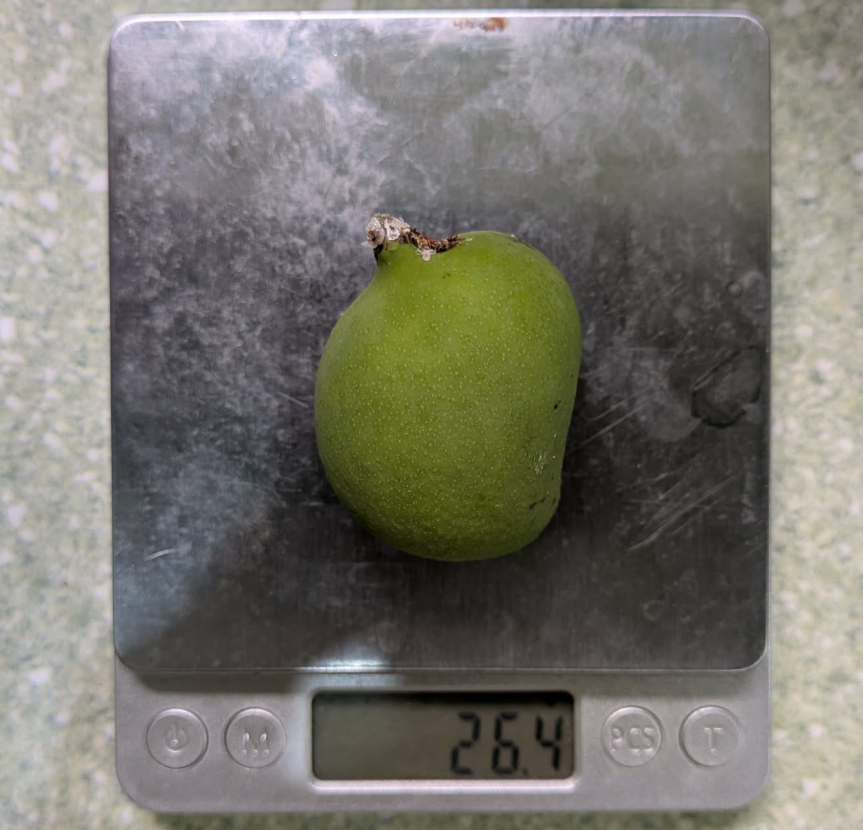
\includegraphics[width=0.85\columnwidth]{graphics/mangoWeighScale.png}
    \caption{Setup demo of Katchamitha mango being weighed using a digital weighing
    scale to collect ground truth mass.}
    \label{fig:weigh_setup}
\end{figure}

\begin{figure}[htbp]
    \centering
    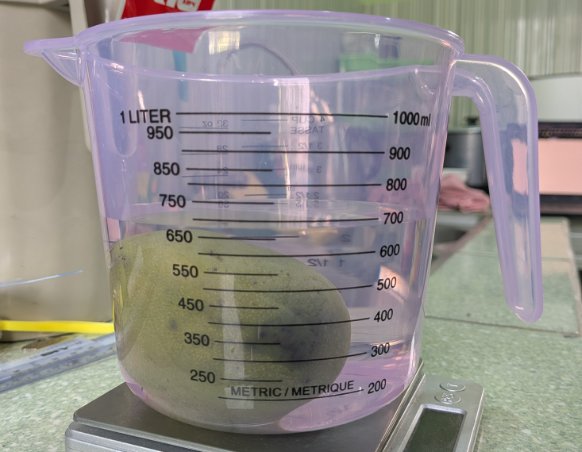
\includegraphics[width=0.85\columnwidth]{graphics/waterDisplacement.png}
    \caption{Experimental setup of the Archimedes water displacement method for measuring the
    physical volume of the mango.}
    \label{fig:water_disp}
\end{figure}

\subsection{Indian Mango Dataset}
The primary dataset consists of 45 Katchamitha (Indian) mango samples collected locally in
Mabalacat City, Pampanga, yielding a total of 243 raw images across six orientations. To
study the effect of scale calibration, the dataset is split: 35 samples (producing 184 raw
and 482 augmented images) are allocated to the uncalibrated pipeline (No ArUco), and 10
samples (producing 59 raw and 158 augmented images) are equipped with ArUco reference markers
for the calibrated pipeline (With ArUco).

To prevent overfitting and expand the training set, data augmentation techniques are employed.
For the segmentation phase, YOLOv11 inherently applies mosaic augmentation, mixup, color adjustments, and geometric transformations. For the orientation classifier, random horizontal
flips, random 15° rotations, and subtle color jitter (brightness, contrast, saturation) are
applied to augment the training set. Conversely, the morphology estimation models are trained
strictly on unaugmented raw images to perfectly preserve the real-world scale and geometric
proportions.

During data annotation, precise polygonal masks are drawn to train the YOLO segmentation model.
Each image is supplemented with attribute metadata tagging, explicitly linking the image to its
orientation, phase, and ground-truth morphological measurements.

\subsection{Data Pipeline Architecture}
The proposed computational pipeline operates in sequential phases, from initial segmentation to
final property estimation, as depicted in the general workflow diagram (Fig.~\ref{fig:general_pipeline}).

\begin{figure*}[htbp]
    \centering
    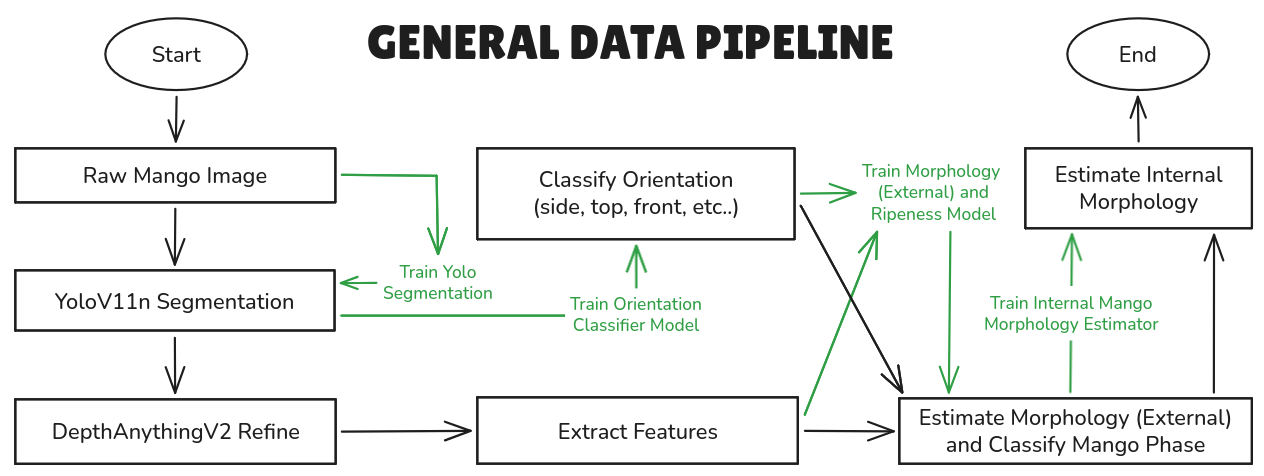
\includegraphics[width=0.85\textwidth]{graphics/pipeline.png}
    \caption{The proposed pipeline architecture showing initial YOLOv11 segmentation,
    DepthAnythingV2 integration to estimate mango orientation, ripeness, and morphology.}
    \label{fig:general_pipeline}
\end{figure*}

\subsubsection{Segmentation Model (RGB + Depth Fusion)}
An input RGB image is processed by a YOLOv11n instance segmentation model to generate an
initial mask separating the mango from the background. Concurrently, the image is passed
through the Depth Anything V2 model (metric version, pre-trained on the Hypersim dataset)
\cite{depth_anything_v2} to produce a high-resolution depth map. The depth map is then fused
with the YOLO mask to refine the boundaries, effectively resolving the green-to-green camouflage
problem \cite{depthcl} (see Fig.~\ref{fig:depth_fusion_ex}).

\begin{figure*}[htbp]
    \centering
    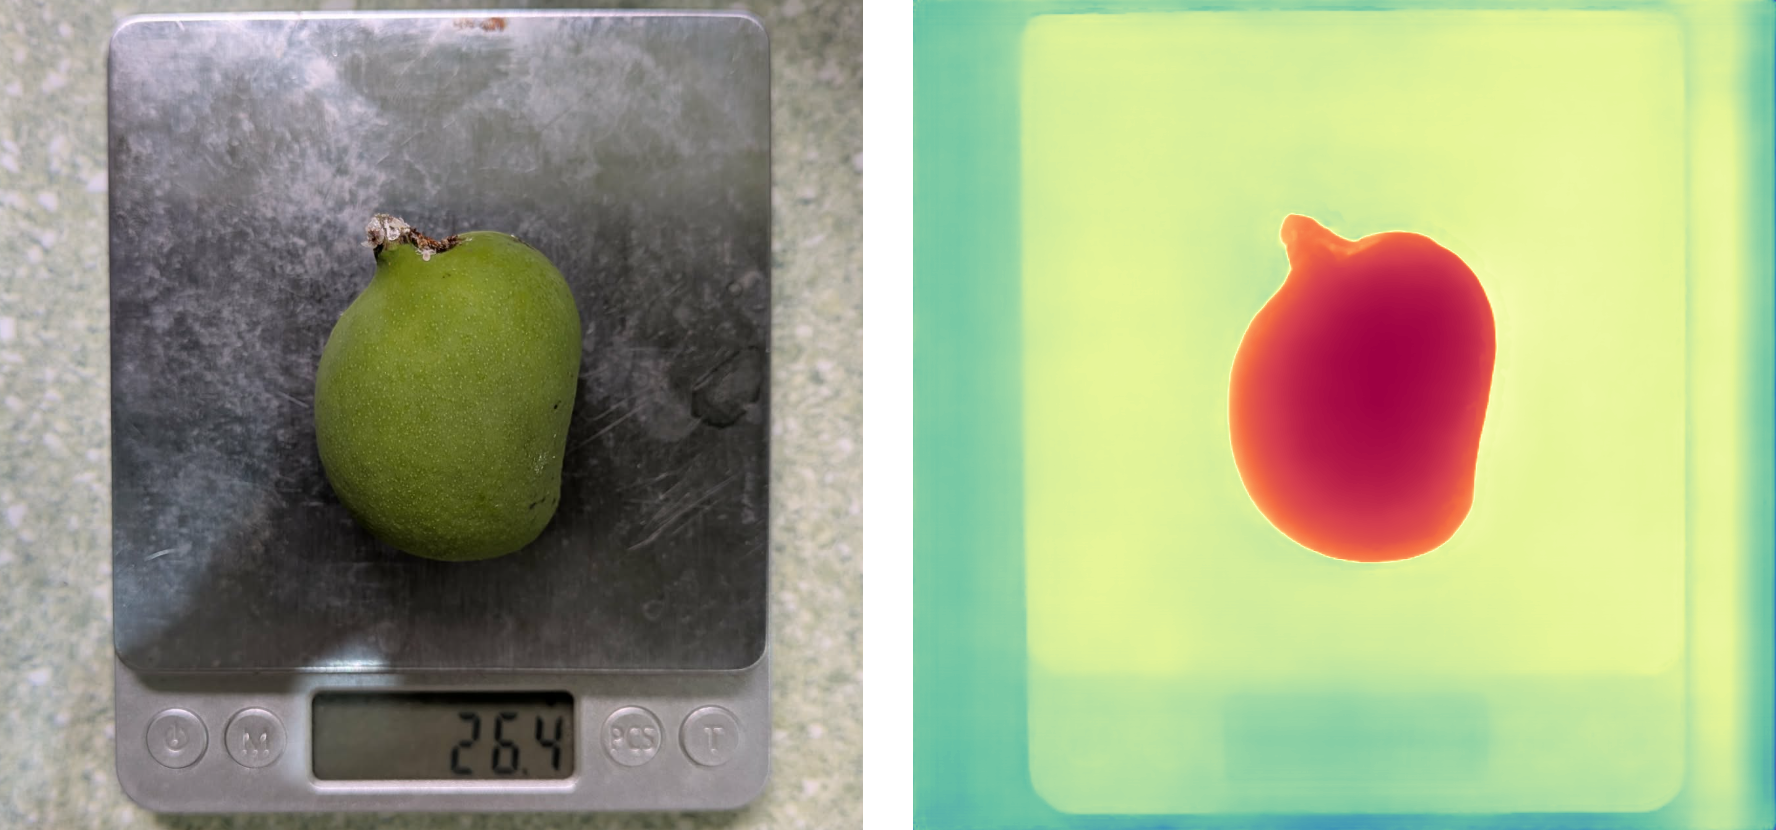
\includegraphics[width=0.85\textwidth]{graphics/depthAnythingV2.png}
    \caption{Visual example of DepthAnythingV2 depth map output.}
    \label{fig:depth_fusion_ex}
\end{figure*}

\subsubsection{ArUco Scale Calibration}
For the calibrated pipeline, an ArUco fiducial marker of known dimensions is placed in the
camera's field of view. The marker is detected, and its pixel width $P_{\text{marker}}$ is used to
calculate the physical scale factor $S_{\text{aruco}}$ (meters per pixel):
\begin{equation}
S_{\text{aruco}} = \frac{W_{\text{marker}}}{P_{\text{marker}}}
\label{eq:scale_factor}
\end{equation}
where $W_{\text{marker}}$ is the known physical width of the marker ($0.05$ m). Using the
camera intrinsic focal length $f$, the absolute distance $Z_{\text{marker}}$ to the marker is
calculated as:
\begin{equation}
Z_{\text{marker}} = f \times S_{\text{aruco}}
\label{eq:depth_calib}
\end{equation}
The absolute metric height $H_{\text{metric}}$ and width $W_{\text{metric}}$ of the mango bounding box are obtained from their pixel-based counterparts $H_{\text{pixel}}$ and $W_{\text{pixel}}$:
\begin{equation}
H_{\text{metric}} = H_{\text{pixel}} \times S_{\text{aruco}}
\label{eq:height_metric}
\end{equation}
\begin{equation}
W_{\text{metric}} = W_{\text{pixel}} \times S_{\text{aruco}}
\label{eq:width_metric}
\end{equation}
Similarly, the projected surface area of the mango in metric units is calculated as:
\begin{equation}
A_{\text{metric}} = A_{\text{pixel}} \times S_{\text{aruco}}^2
\label{eq:area_metric}
\end{equation}

\subsubsection{Feature Extraction}
From the refined mask and depth map, robust geometric and color features are extracted:
\begin{itemize}
    \item \textbf{Geometric Features:} In the uncalibrated pipeline, where absolute metric coordinates are unavailable, scale-invariant ratios are utilized to bypass distance-based fluctuations \cite{depthanythingv2}:
    \begin{itemize}
        \item \textit{Dimension Ratios:} Height-to-Width, Width-to-Depth, and Height-to-Depth.
        \item \textit{Solidity:} The ratio of the estimated mango volume (derived from a 3D
point cloud projected from the depth map) to the volume of its 3D bounding box convex
hull ($W \times H \times T$).
        \item \textit{Thickness:} Maximum and Mean thickness of the visible half of the mango
        derived from the depth gradients.
        \item \textit{Curvature:} Mean and standard deviation of surface curvature, estimated
        using the spatial gradients of the depth map to assess surface normal variations.
    \end{itemize}
    In the calibrated pipeline, these ratios are supplemented with the absolute dimensions
    $H_{\text{metric}}$, $W_{\text{metric}}$, and $A_{\text{metric}}$ derived from
    Eq.~\ref{eq:height_metric}--\ref{eq:area_metric}.
    \item \textbf{Color Features:} Color characteristics are extracted using the CIELab color
    space, which closely approximates human vision and is highly effective for maturity
    assessment in green fruits. The average green-red ($a^*$) axis and average blue-yellow
    ($b^*$) axis values are calculated to inform the ripeness and density models.
\end{itemize}

\subsubsection{Orientation Classification}
Because the physical profile of a mango changes drastically depending on the camera's viewing
angle, an intermediate Orientation Classification Model classifies the input image into one of
five orientations (Side, Top, Bottom, Front, or Back). This routing layer ensures that the
subsequent feature vectors are passed to the correct, specialized morphology estimation pipeline.

The classifier is implemented as a fine-tuned \textbf{MobileNetV3-Small} convolutional neural network (CNN) pre-trained on ImageNet. The final classifier head is replaced with a 5-class linear layer. Training employs an AdamW optimizer ($lr=1\times10^{-4}$, weight decay $1\times10^{-4}$) with a cosine annealing learning-rate schedule over 15 epochs. Input images are first cropped to the YOLO segmentation mask bounding box (with 5\% padding), resized to $224\times224$ pixels, and normalized with ImageNet statistics. To ensure that all five orientation classes can be robustly identified regardless of how the fruit is held, the model is trained on the full 45-mango dataset (all 640 augmented images) and evaluated via a Group Shuffle Split ($20\%$ test, grouped by mango ID) to guarantee that no test image shares a mango subject with the training set.

\subsubsection{Ripeness and Morphology Estimation}
The final phase employs an ensemble of machine learning algorithms. A Random Forest classifier evaluates the extracted color and geometric features to determine the ripening phase (ripe or unripe). Simultaneously, a multi-output regression model (specifically tuned for the recognized orientation) processes the scale-invariant ratios to estimate the absolute dimensions, volume, and weight of both the mango and its internal bone. The density is explicitly calculated using the formula $\rho = \frac{m}{V}$. Finally, the model outputs the estimated stone-to-flesh ratio, providing a comprehensive, non-destructive morphological profile of the fruit.
